\documentclass[12pt]{scrartcl}

\usepackage[american]{babel}

\usepackage{graphicx}
\graphicspath{{images/}}

\usepackage{paralist}
\usepackage{csquotes}
\usepackage[T1]{fontenc}
\usepackage{lmodern}

\usepackage{geometry}
% \geometry{a4paper,body={5.8in,9in}}
\geometry{a4paper}

\usepackage{amsmath, amsfonts, amssymb}
\usepackage{placeins}
\usepackage{subcaption}

\usepackage{setspace}

\setlength{\parindent}{0pt}
%
%%%%%%%%%%%%%%%%%%%%%%%%%%%%%%%%%%%%%%
% ab hier steht der eigentliche Text:
\begin{document}
\title{Thesis Title}
\subtitle{Bachelor Thesis Proposal \& Work Plan}
% bei Masterarbeit ggf. ändern
\author{First Name + Name\\ \small{matriculation number: xxxxxxx}\\ \small{mail-address}}
\date{\today}
\maketitle

\section{Motivation}\label{sec:motivation}

\section{Task Objectives}\label{sec:task-objectives}

\section{Task Description}\label{sec:task-description}

\section{Time-Schedule and Subtasks}\label{sec:schedule-and-subtasks}

% % %
\begin{figure}[!ht]
	\centering
	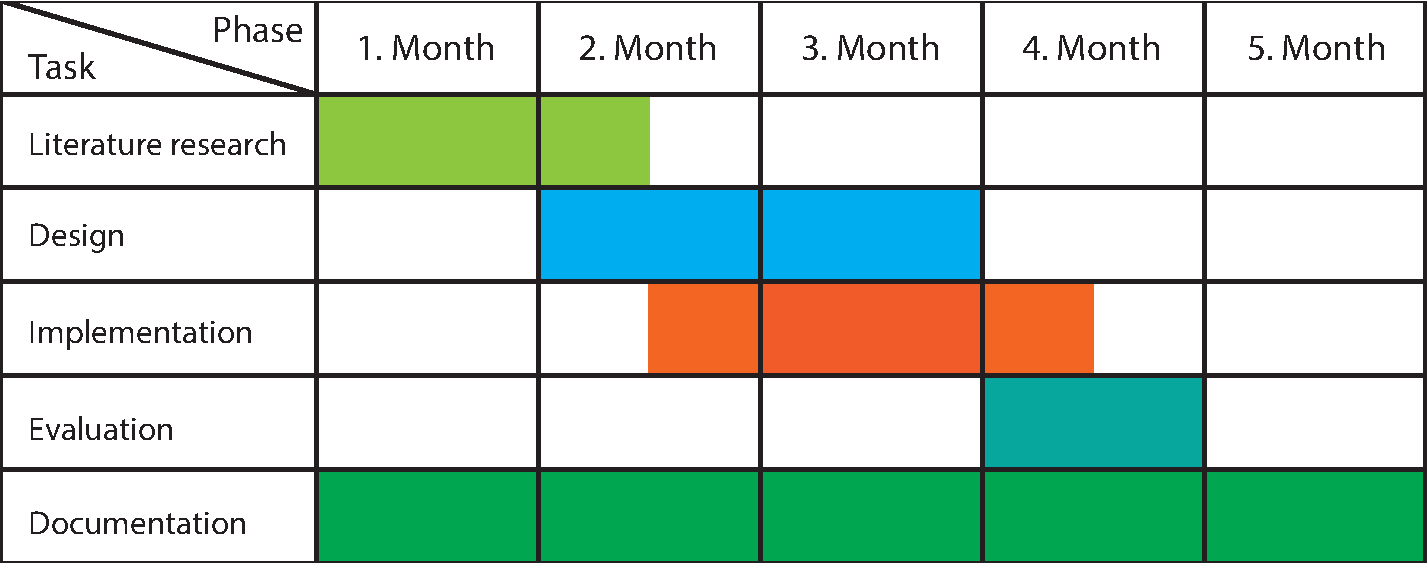
\includegraphics[width=.9\textwidth]{timeschedule}
	\caption{Sketch of the time schedule for the work on the thesis}
	\label{fig:time-schedule}
\end{figure}
% % %
\section{Initial Document Structure}\label{sec:doc-structure}
\begin{enumerate}
	\item Introduction
	\item ...
\end{enumerate}
\newpage
\bibliography{literature}
\bibliographystyle{myalphadin}

\vspace{6cm}

\begin{center}
     \begin{tabular}{l p{0.1\textwidth} r}
       \cline{1-1} \cline{3-3}
       \begin{minipage}[t]{0.4\textwidth}
         \centering
         Supervisor)\\(Titel Vorname Nachname)
         \end{minipage}
&
         \begin{minipage}[t]{0.2\textwidth}
         \end{minipage}
&
         \begin{minipage}[t]{0.4\textwidth}
           \centering
           Student(in)\\(Vorname Nachname)
         \end{minipage}
     \end{tabular}
\end{center}

\end{document}
